\section{Design}
\label{design}
\begin{figure}[!t]
        \centering
  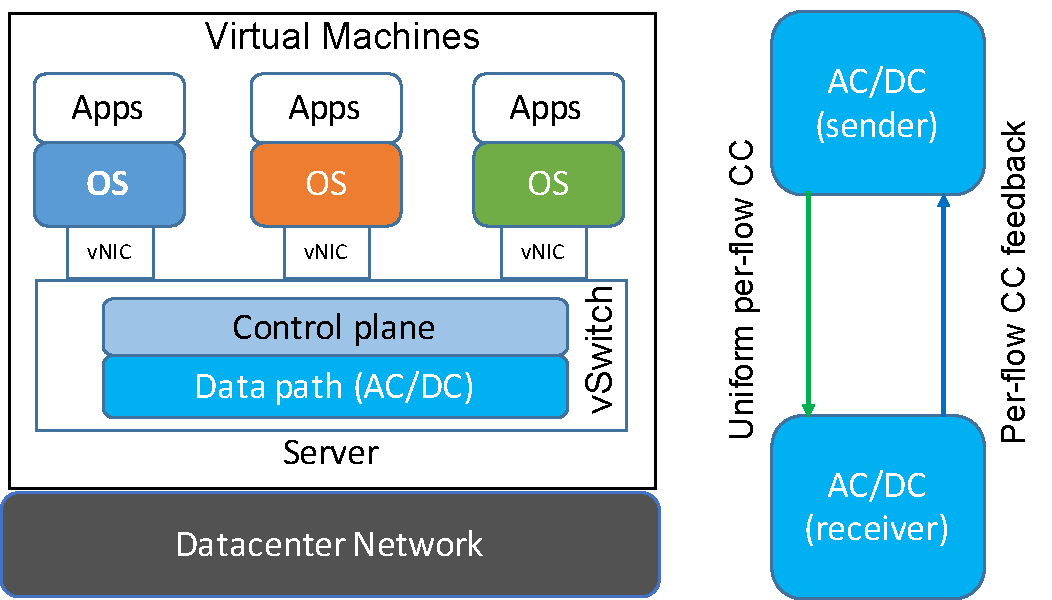
\includegraphics[width=0.7\textwidth]{acdctcp/figures/acdc_highlevel.pdf}
        \caption{\acdc{} high-level architecture.}
        \label{acdc_highlevel}
\end{figure}

This section provides an overview of~\acdc{}'s design. First, we show how basic
congestion control state can be inferred in the vSwitch. Then we study
how to implement DCTCP. Finally, we discuss how to enforce congestion
control in the vSwitch and provide a brief overview of how per-flow differentiation
can be implemented.


\begin{figure}[th]
        \centering
  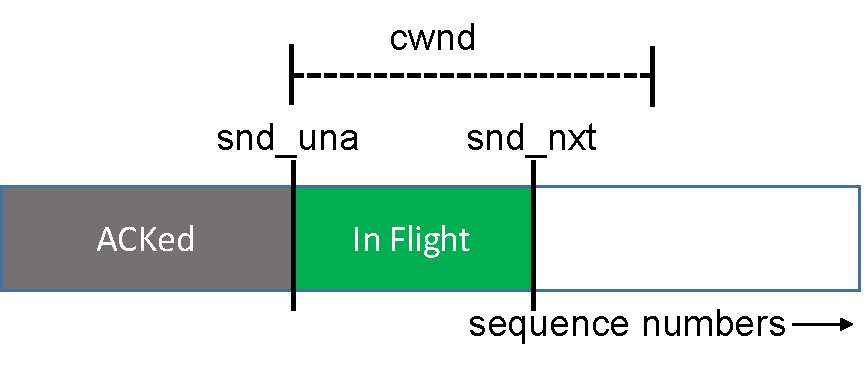
\includegraphics[width=0.7\textwidth]{acdctcp/figures/tcp-state-new.pdf}
        \caption{Variables for TCP sequence number space.}
        \label{tcpstate}
\end{figure}
\subsection{Obtaining Congestion Control State}
\label{ss:tcpstate}
Figure~\ref{acdc_highlevel} shows the high-level structure of \acdc{}. Since it is
implemented in the datapath of the vSwitch, all traffic can be monitored. The sender
and receiver modules work together to implement per-flow congestion control (CC).

We first demonstrate how congestion control state can be inferred.
Figure~\ref{tcpstate} provides a visual of the TCP sequence number space. The {\tt snd\_una} variable is the first byte
that has been sent, but not yet ACKed. The {\tt snd\_nxt} variable is the 
next byte to be sent. Bytes between {\tt snd\_una} and {\tt snd\_nxt} are in flight.
The largest number of packets that can be sent and unacknowledged is bounded by \cwnd{}.
{\tt snd\_una} is simple to update: each ACK contains an acknowledgement number ({\tt ack\_seq}), and 
{\tt snd\_una} is updated when {\tt ack\_seq} $>$ {\tt snd\_una}.
When packets traverse the vSwitch from the VM, {\tt snd\_nxt} is updated if the sequence
number is larger than the current {\tt snd\_nxt} value.
Detecting loss is also relatively simple. If {\tt ack\_seq $\le$ snd\_una}, then
a local {\tt dupack} counter is updated. Timeouts can be inferred when {\tt snd\_una $<$ snd\_nxt}
and an inactivity timer fires. The initial~\cwnd{} is set to a default value of 10~\cite{RFC6928}. 
With this state, the vSwitch can determine appropriate~\cwnd{} values for canonical
TCP congestion control schemes.
%More advanced congestion control techniques that rely on timestamps, round-trip times, SACKs or 
%FACKs can also be implemented. 
We omit additional details in the interest of space. 



\subsection{Implementing DCTCP}
%\begin{figure}[!t]
%        \centering
%  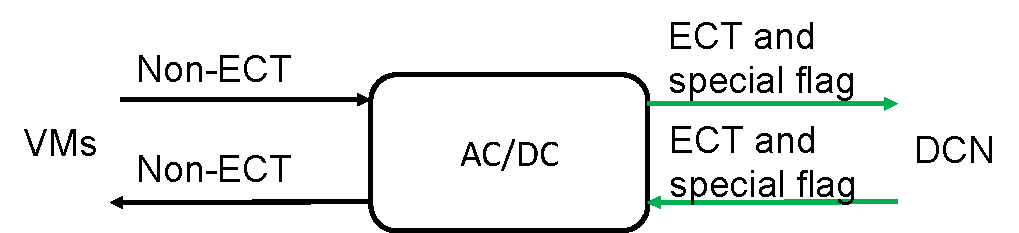
\includegraphics[width=0.45\textwidth]{acdctcp/figures/acdc_ECT_marking.pdf}
%        \caption{Simple stateless ECT marking in \acdc{}. 
%		Turn all intra-DC TCP packets in the fabric into ECT.}
%        \label{acdc_ect_marking}
%\end{figure}

%\begin{figure}[!t]
%        \centering
%  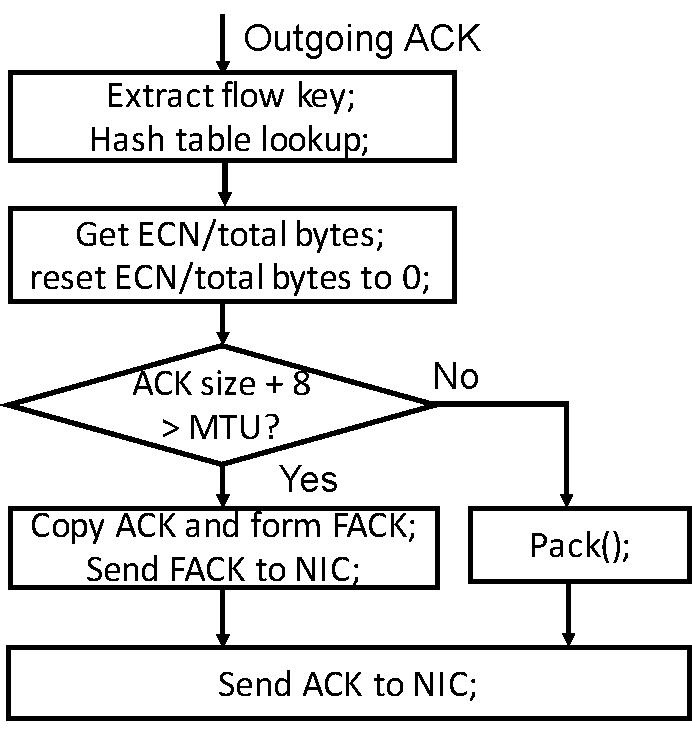
\includegraphics[width=0.25\textwidth]{acdctcp/figures/carry_ecn_info.pdf}
%        \caption{Carrying the congestion information back. 
%		Being compatible with TSO and minimizing CPU and traffic overhead.}
%        \label{acdc_carry_ecn_info}
%\end{figure}

This section discusses how to obtain DCTCP state and perform its congestion control.


\tightparagraph{ECN marking} 
DCTCP requires flows to be ECN-capable, but the VM's TCP stack may not support ECN.
Thus, all egress packets are marked to be ECN-capable on the sender module. 
When the VM's TCP stack does not support ECN, all ECN-related bits on ingress packets are stripped at the sender
and receiver modules in order to preserve the original TCP settings. When the VM's TCP
stack does support ECN, the~\acdc{} modules strip the {\tt congestion encountered} 
bits in order to prevent the VM's TCP stack from decreasing rates too aggressively
(recall DCTCP adjusts~\cwnd{} proportional to the fraction of congested packets, while traditional schemes conservatively reduce~\cwnd{} by half). A reserved bit in
the header is used to determine if the VM's TCP stack originally 
supported ECN.
%Algorithm~\ref{alg:non-ect-to-ect} changes non-ECT packets into ECT packets
%in the virtual switch before the packets enter the fabric and
%change them back when they arrive at the destination virtual switch.
%$p.pretendECT$ is set or cleared by flipping the 2nd bit of the 3 reserved bits in TCP header.
%After applying this algorithm, all TCP packets traversing the network appear to be ECT packets.
%So the ECT and non-ECT coexistence issue is solved.
%Also, because we change non-ECT back at the destination virtual switch,
%so TCP is not aware of such a transformation and \acdc{} does not break any TCP connections or applications.
%Algorithm~\ref{alg:non-ect-to-ect} leverages hardware checksumming feature in the NIC implicitly to reduce CPU overhead.
%\todo{how to add comment in this algorithm?}.
%
%
%\begin{algorithm}[t]
%\caption{ECT marking in \acdc{}}
%\label{alg:non-ect-to-ect}
%\begin{algorithmic}[1]
%%\STATE \Comment{packet $p$ is TCP packet}
%\IF{$p$ is going to the network}
%\IF{$p$ is non-ECT}
%\STATE change $p$ to ECT by modifying IP header
%\STATE set $p.pretendECT$
%%\STATE set the 2nd bit of the 3 reserved bits in TCP header to 1
%\ENDIF
%\ELSIF{$p$ is coming from the network}
%\IF{$p$ is non-ECT and $p.pretendECT$ is set}
%\STATE change $p$ back to non-ECT by modifying IP header
%\STATE clear $p.pretendECT$
%%\STATE clear the 2nd bit of the reserved bits
%\ENDIF
%\ENDIF
%\end{algorithmic}
%\end{algorithm}
%

\tightparagraph{Obtaining ECN feedback}
In DCTCP, the fraction of packets experiencing congestion needs to be reported to the sender. 
%DCTCP relays this information from the destination to the sender by essentially modulating data
%in the ACK reporting scheme. Sender and receiver agree on an ACK state-machine that effectively 
%communicates how many packets were received with ECN vs how many were not. Because the TCP stack
%in the VM may not be DCTCP, we do not want to rely on the ACK modulation scheme. 
Since the VM's TCP stack may not support ECN, the~\acdc{} receiver module monitors
the total and ECN-marked bytes received for a flow. Receivers piggy-back the
reported totals on ACKs by adding an additional 8 bytes as a TCP Option. This is called 
a Piggy-backed ACK (PACK). The PACK is created by moving the IP and TCP headers into
the ACK packet's {\tt skb} headroom~\cite{kernel-skb}. The totals are inserted into the vacated space and the memory
consumed by the rest of the packet (\ie{}the payload) is left as is. The IP header checksum, IP packet length and TCP Data Offset fields are recomputed and the 
TCP checksum is calculated by the NIC. The PACK option is stripped at the
sender so it is not exposed to the VM's TCP stack. 

If adding a PACK creates a packet larger than the MTU, the NIC offload feature (\ie{}TSO)
will replicate the feedback information over multiple packets, which skews the feedback.
Therefore, a dedicated feedback packet called a Fake ACK (FACK) is sent when the MTU
will be violated. The FACK is sent in addition to the real TCP ACK.
FACKs are also discarded by the sender after logging the included
data. In practice, most feedback takes the form of PACKs.

%
%\begin{algorithm}[t]
%\caption{Carrying the congestion information back}
%\label{alg:outgoing}
%\begin{algorithmic}[1]
%%\STATE flow\_key $\leftarrow$ \{dstip, srcip, dstport, srcport\}
%%\STATE ack\_entry $\leftarrow$ rcv\_ack\_hashtbl\_lookup(flow\_key)
%%\STATE end\_seq $\leftarrow$ ntohl(tcp.seq) + tcp.data\_len
%%\IF{after(end\_seq, ack\_entry.snd\_nxt)}
%%       \STATE ack\_entry.snd\_nxt $\leftarrow$ end\_seq
%%\ENDIF
%%\IF{tcp.ack}
%\IF{outgoing skb is a TCP ACK}
%\STATE flow\_key $\leftarrow$ \{dstip, srcip, dstport, srcport\}
%\STATE entry $\leftarrow$ rcv\_data\_hashtbl\_lookup(flow\_key)
%        \IF{entry.total\_bytes > 0}
%                \STATE ecn\_bytes $\leftarrow$ entry.ecn\_bytes
%                \STATE total\_bytes $\leftarrow$ entry.total\_bytes
%                \STATE entry.ecn\_bytes $\leftarrow$ 0
%                \STATE entry.total\_bytes $\leftarrow$ 0
%        \ENDIF
%        \IF{total\_bytes > 0}
%                \IF{skb.data\_len < (MTU -- HEADROOM)}
%                        \STATE skb $\leftarrow$ ovs\_pack(skb, ecn\_bytes, total\_bytes)
%                \ELSE
%                        \STATE fack $\leftarrow$ ovs\_fack(skb, ecn\_bytes, total\_bytes)
%                \ENDIF
%        \ENDIF
%\ENDIF
%\IF{fack != NULL}
%        \STATE sendtoNIC(fack)
%\ENDIF
%\STATE sendtoNIC(skb)
%\end{algorithmic}
%\end{algorithm}
%

\begin{figure}[!t]
        \centering
  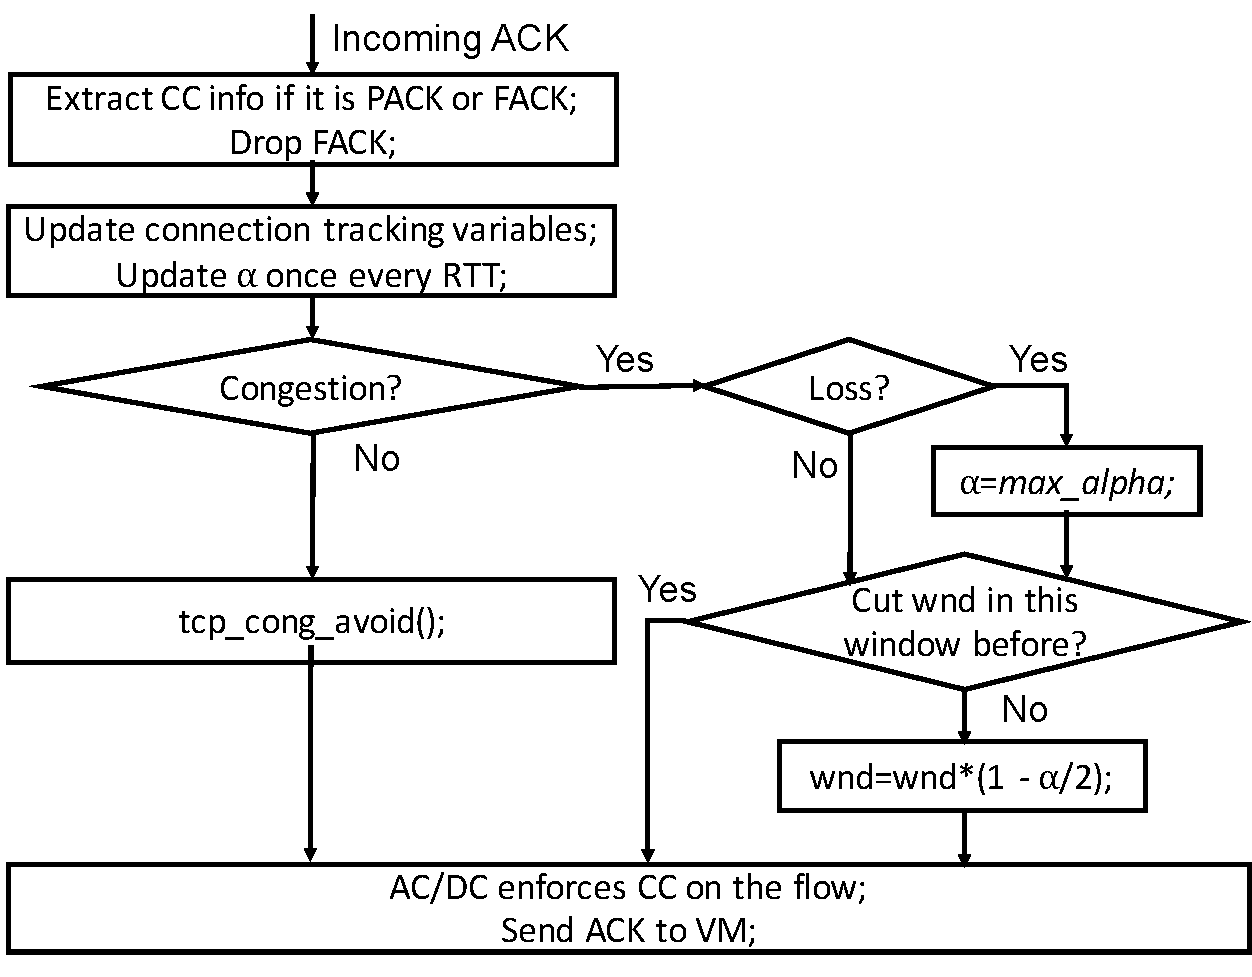
\includegraphics[width=0.7\textwidth]{acdctcp/figures/acdc_cc.pdf}
        \caption{DCTCP congestion control in \acdc{}.}
        \label{acdc_cc}
\end{figure}
\tightparagraph{DCTCP congestion control} 
Once the fraction of ECN-marked packets is obtained, implementing DCTCP's logic is straightforward.
Figure~\ref{acdc_cc} shows the high-level design. 
First, congestion control (CC) information is extracted from FACKs and PACKs. Connection tracking
variables (described in \sref{ss:tcpstate}) are updated based on the ACK. The variable
$\alpha$ is an EWMA of the fraction of packets that experienced congestion and is updated roughly
once per RTT. If congestion was not encountered (no loss or ECN), then {\tt tcp\_cong\_avoid} advances~\cwnd{}
based on TCP New Reno's algorithm, using slow start or congestion avoidance as needed. If congestion was
experienced, then~\cwnd{} must be reduced. DCTCP's instructions indicate the window should
be cut at most once per RTT.
Our implementation closely tracks the Linux source code, and
additional details can be referenced externally~\cite{dctcp,ietf-tcpm-dctcp}.


%\begin{algorithm}[!tbh]
%\caption{Congestion control in \acdc{}}
%\label{alg:incoming}
%\begin{algorithmic}[1]
%\IF{incoming skb is a TCP ACK}
%\STATE initialize is\_rack, is\_pack and is\_fack
%\STATE flow\_key $\leftarrow$ \{srcip, dstip, srcport, dstport\}
%\STATE entry $\leftarrow$ rcv\_ack\_hashtbl\_lookup(flow\_key)
%\IF{is\_pack or is\_fack}
%        \STATE unpack and extract ecn\_bytes and total\_bytes
%        \STATE update(entry.ecn\_bytes, ecn\_bytes)
%        \STATE update(entry.total\_bytes, total\_bytes)
%\ENDIF
%\IF{is\_rack or is\_pack}
%        \STATE acked $\leftarrow$ tcp.ack\_seq -- entry.snd\_una
%        \STATE entry.snd\_una $\leftarrow$ tcp.ack\_seq
%        \IF{duplicated ACK}
%                \STATE entry.dupack\_cnt++
%        \ENDIF
%        \STATE dctcp\_update\_alpha(entry)
%        \IF{acked > 0}
%                \IF{may\_raise\_rwnd(entry)}
%                        \STATE tcp\_cong\_avoid(entry, acked)
%                \ENDIF
%        \ENDIF
%\ENDIF
%\IF{entry.dupack\_cnt >= 3 or ecn\_bytes > 0}
%        \IF{entry.dupack\_cnt >= 3}
%                \STATE entry.alpha $\leftarrow$ MAX\_ALPHA
%                \STATE entry.loss $\leftarrow$ true
%        \ENDIF
%        \IF{may\_reduce\_rwnd(entry)}
%                \STATE entry.ssthresh $\leftarrow$ dctcp\_ssthresh(ack\_entry)
%                \STATE entry.rwnd $\leftarrow$ min(RWND\_MIN, entry.ssthresh)
%                \STATE entry.reduced $\leftarrow$ true
%        \ENDIF
%\ENDIF
%\IF{is\_rack or is\_pack}
%        \STATE tcp.window $\leftarrow$ min(tcp.window, entry.rwnd)
%\ENDIF
%\IF{is\_fack}
%        \STATE drop(skb)
%\ENDIF
%\ENDIF
%\end{algorithmic}
%\end{algorithm}
%

\subsection{Enforcing Congestion Control}
\label{ss:enforce}
There must be a mechanism to ensure a VM's TCP flow adheres to the 
congestion control window size determined in the vSwitch.
Luckily, TCP provides built-in functionality that can be reprovisioned for~\acdc{}. Specifically,
TCP's flow control allows a receiver to advertise the amount of data it is willing to process via
a receive window (\rwnd{}).~\crs{Similar to other works~\cite{Kalampoukas02,Spring00}, the vSwitch overwrites~\rwnd{} with its calculated~\cwnd{}}.
In order to preserve TCP semantics, this value is overwritten only when it is smaller than the packet's original~\rwnd{}.
The VM's flow then uses $min(\cwnd{},\rwnd{})$ to limit how many packets it can send.

This enforcement scheme must be compatible with TCP receive window scaling to work in practice.
Scaling ensures~\rwnd{} does not become an unnecessary upper-bound in high bandwidth-delay networks
and provides a mechanism to left-shift~\rwnd by a window scaling factor~\cite{RFC1323}. 
The window scaling factor is negotiated during TCP's handshake, so~\acdc{} monitors handshakes
to obtain this value. Calculated congestion windows are adjusted accordingly.
TCP receive window auto-tuning~\cite{semke1998automatic} manages buffer state
and thus is an orthogonal scheme~\acdc{} can safely ignore.

Ensuring a VM's flow adheres to~\rwnd{} is relatively simple. The vSwitch calculates a new congestion 
window every time an ACK is received. This value provides a bound on the number of bytes the VM's flow
is now able to send. VMs with unaltered TCP stacks will naturally follow our enforcement scheme because the stacks
will simply follow the standard. Flows that circumvent the standard can be policed by dropping
excess packets not allowed by the calculated congestion window, which incentivizes tenants to respect the standard.

While simple, this scheme provides a surprising amount of flexibility. For example, TCP enables
a receiver to send a TCP Window Update to update~\rwnd{}~\cite{RFC5681}.~\acdc{}
can create these packets to update windows without relying on ACKs.
Additionally, the sender module can generate duplicate ACKs to to trigger retransmissions. This is useful when 
the VM's TCP stack has a larger timeout value than~\acdc{} (\eg{}small timeout values
have been recommended for incast~\cite{vasudevan2009safe}). 
%In this case, the vSwitch can send three dup-ACKs (with
%an appropiate~\rwnd{}) to trigger the VM's TCP flow to retransmit.
% EJR-- put back in for camera ready?
\crs{
Another useful feature is when~\acdc{} allows a TCP stack to send {\em more} data. This can occur when
a VM TCP flow aggressively reduces its window when ECN feedback is received. By removing ECN feedback
in~\acdc{}, the VM TCP stack won't reduce~\cwnd{}. 
In a similar manner, DCTCP limits loss more effectively than aggressive TCP stacks. Without loss
or ECN feedback, VM TCP stacks grow~\cwnd{}. This causes~\acdc{}'s~\rwnd{} to become the limiting window, and thus~\acdc{} can 
increase a flow's rate instantly when~\rwnd{} $<$ \cwnd{}. Note, however,~\acdc{} cannot force
a connection to send more data than the VM's~\cwnd{} allows.
}

Another benefit of~\acdc{} is that it scales in the number of flows.
Traditional software-based rate limiting schemes, like Linux's Hierarchical Token Bucket, 
incur high overhead due to frequent interrupts and contention~\cite{radhakrishnan2014senic} and
therefore do not scale gracefully. NIC or switch-based rate limiters are low-overhead, but typically
only provide a handful of queues. Our enforcement algorithm does not rate limit or buffer packets because it exploits TCP
flow control. Therefore, rate limiting schemes can be used at a coarser granularity (\eg{}VM-level).


~\crs{
Finally, we outline~\acdc{}'s limitations. 
Since~\acdc{} relies on sniffing traffic, schemes that encrypt TCP headers (\eg{}IPSec) are not supported. Our implementation only supports TCP, but we believe it can be extended to handle UDP similar to
prior schemes~\cite{shieh2011sharing,jeyakumar2013eyeq}.
Implementing per-flow DCTCP-friendly UDP tunnels and studying its impact remains future work, however. And finally, 
while MPTCP supports per-subflow~\rwnd{}~\cite{RFC6824}, it is not included in our case study and a more detailed analysis
is future work.
}
 


%\tightparagraph{Compatible with receive window auto-tuning and window scaling}
%TCP receive window auto-tuning~\cite{semke1998automatic,receive-auto-runing} is a commonly used feature 
%in modern TCP stacks. It is enabled by default in recent Linux and Windows distributions.
%Receive window auto-tuning was proposed to automatically 
%set socket buffer size based on network conditions to 
%improve network performance while optimizing the memory usage by TCP connections.
%Because \acdc{} overwrites the real \rwnd{} value embedded in TCP ACK header 
%only when \acdc{}'s running \rwnd{} is smaller than 
%the real \rwnd{}, thus \acdc{} does not break the correctness of TCP semantics 
%and is compatible with receive window auto-tuning.
%

\begin{figure}[t]
        \centering
        \begin{subfigure}[b]{0.45\textwidth}
                \centering
                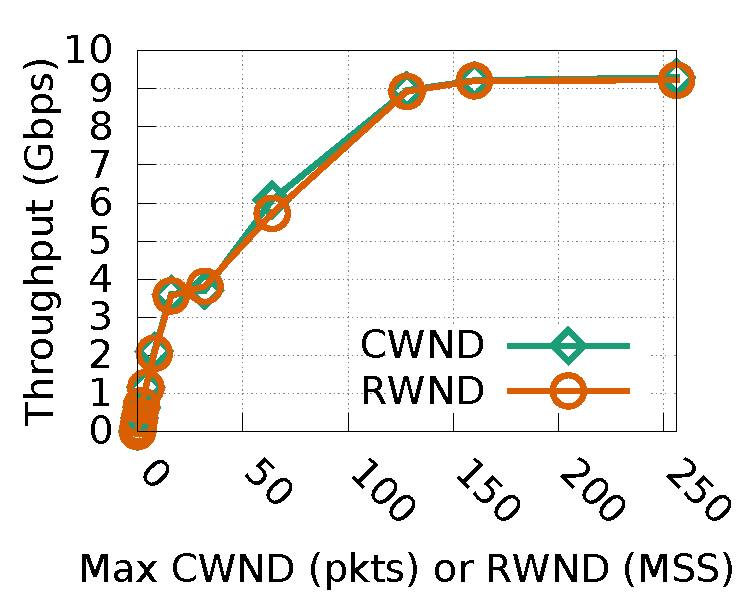
\includegraphics[width=\textwidth]{acdctcp/figures/new_enforce/new_tput_cwnd_rwnd_cubic_15k.pdf}
                \caption{MTU = 1.5KB.}
                \label{effectiveness_15k}
        \end{subfigure}
        \begin{subfigure}[b]{0.45\textwidth}
                \centering
                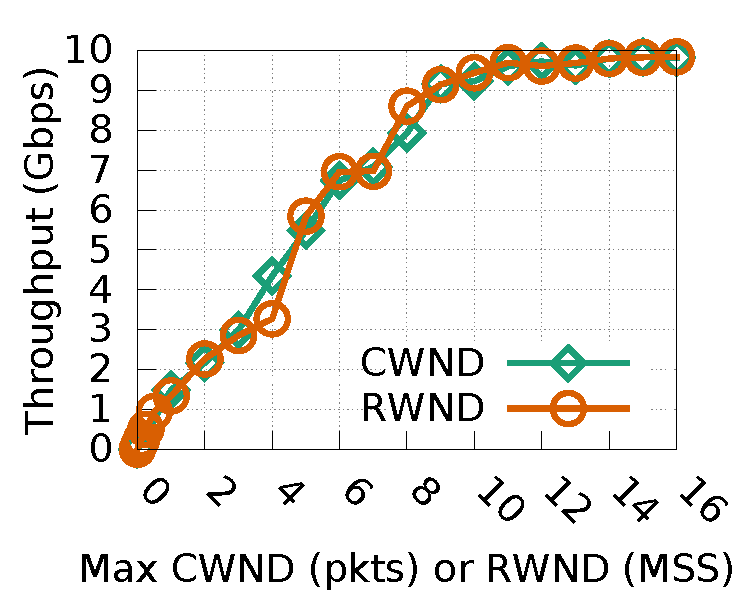
\includegraphics[width=\textwidth]{acdctcp/figures/new_enforce/new_tput_cwnd_rwnd_cubic_9k.pdf}
                \caption{MTU = 9KB.}
                \label{effectiveness_9k}
        \end{subfigure}
        \caption{Using \rwnd{} can effectively control throughput.}
                %Experiments are conducted on a 10G testbed. TCP CUBIC but New Reno shows similar results.
                %Linux 3.18.0. We control maximal \rwnd{} value by modifying the receiver's advertised window size in TCP ACKs
                %in the Open vSwitch. We control maximal \cwnd{} by specifying ``snd\_cwnd\_clamp" value in Linux TCP.}
        \label{rwnd_effectiveness}
\end{figure}
\subsection{Per-flow Differentiation}
\label{ss:cc-qos}
\acdc{} can assign different congestion control algorithms
on a per-flow basis. This gives administrators additional flexibility and control by 
assigning flows to specific congestion control algorithms based on policy.
For example, flows destined to the WAN may be assigned CUBIC and flows destined within the
datacenter may be set to DCTCP. 

Administrators can also enable per-flow bandwidth allocation schemes.
A simple scheme enforces an upper-bound
on a flow's bandwidth. Traditionally, an upper-bound on a flow's~\cwnd{} can be
specified by the parameter {\tt snd\_cwnd\_clamp} in Linux.~\acdc{} can provide similar functionality
by bounding~\rwnd{}. Figure~\ref{rwnd_effectiveness} shows the behavior is equivalent. This 
graph can also be used to convert a desired upper-bound on bandwidth into an appropriate maximum~\rwnd{} (the
graph is created on an uncongested link to provide a lower bound on RTT). 

In a similar fashion, administrators can assign different bandwidth priorities to flows by altering the 
congestion control algorithm. Providing differentiated services via congestion control has 
been studied~\cite{Venkataramani2002tcpnice,shieh2011sharing}. Such schemes are useful because networks
typically contain only a limited number of service classes and bandwidth may need to be allocated on
a finer-granularity. We propose a unique priority-based congestion control algorithm for~\acdc{}.
Specifically, DCTCP's congestion control algorithm is modified to incorporate a priority, $\beta \in [0,1]$:
\begin{equation}
rwnd = rwnd (1 - (\alpha - \frac{\alpha{}\beta}{2}))
\label{eqn:cc-qos}
\end{equation}
Higher values of $\beta$ give higher priority. 
When $\beta{}=1$, Equation~\ref{eqn:cc-qos} simply converts to DCTCP congestion control. When
$\beta{}=0$, flows aggressively back-off (\rwnd{} is bounded by 1 MSS to avoid starvation). This equation
alters multiplicative decrease instead of additive increase because increasing~\rwnd{} 
cannot guarantee the VM flow's~\cwnd{} will allow the flow to increase its sending rate.

%subsection{How to keep low overhead?}
%Move to Implementation?
%Connection tracking~\cite{ayuso2006netfilter,ovs-conntrack}.
%
%\subsection{How is it complimentary to other schemes?}
%Like bandwidth allocation.
%
%~\eric{Should we talk about how we can actually increase rate of VM TCP?}
%


%In history, TCP used packet loss as the signal of network congestion. 
%But, using packet loss as the signal can not meet the performance demand of datacenter environment 
%due to high queueing latency and frequent packet losses. Packet loss-based congestion control 
%can work reasonably well for large data transfers but does harm time-critical RPCs. 
%Thus, new congestion control algorithms designed for datacenter networks were proposed. 
%They can be classified into 2 categories: Explicit Congestion Notification (ECN)-based and 
%latency-based. The most straightforward way is to treat ECN as packet loss and cut congestion 
%window before network queue built up and packet loss happens---but this can harm flow throughput. 
%DCTCP improves this by cut window properly based on the portion of marked packets and 
%gives high throughput for large flows and low latency for mice flows. 
%Latency-based congestion control such as TCP-NV, TIMELY, DX use the end-to-end latency 
%as the signal of network congestion. Compared with ECN-based approach, latency is a more 
%prevalent signal for congestion (i.e., does not need ECN capability on the switches). 
%But the challenge of such approaches is to find ways to combat with latency measurement noise 
%caused by TSO, LRO and interrupt coalescence.
%


%\begin{figure}[t]
%        \centering
%        \begin{subfigure}[b]{0.225\textwidth}
%                \centering
%                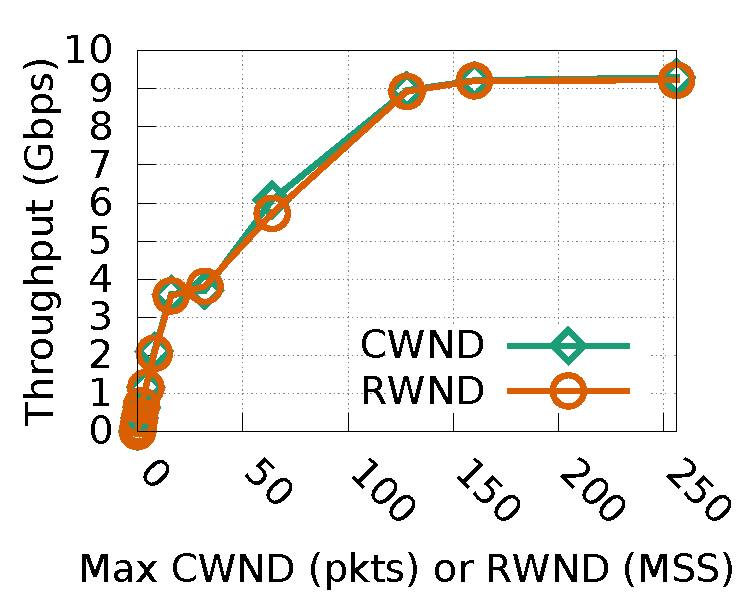
\includegraphics[width=\textwidth]{acdctcp/figures/new_enforce/new_tput_cwnd_rwnd_cubic_15k.pdf}
%                \caption{MTU = 1.5KB.}
%                \label{effectiveness_15k}
%        \end{subfigure}
%        \begin{subfigure}[b]{0.225\textwidth}
%                \centering
%                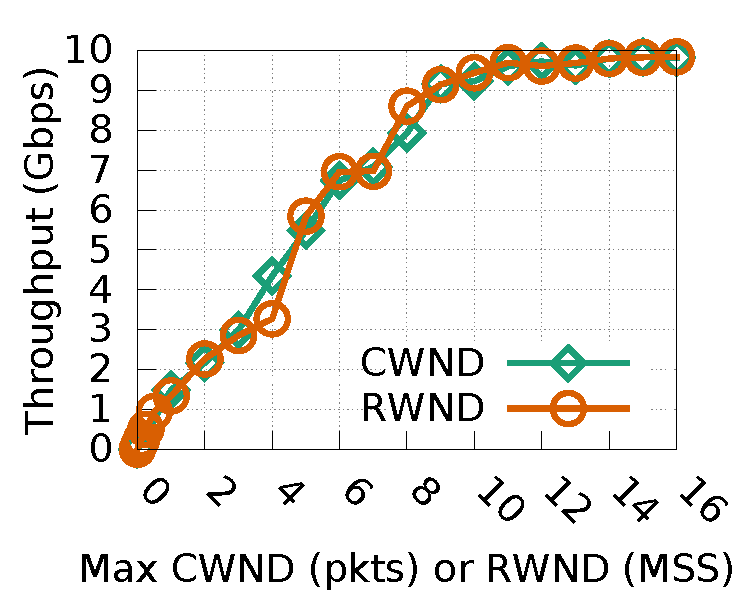
\includegraphics[width=\textwidth]{acdctcp/figures/new_enforce/new_tput_cwnd_rwnd_cubic_9k.pdf}
%                \caption{MTU = 9KB.}
%                \label{effectiveness_9k}
%        \end{subfigure}
%        \caption{Using \rwnd{} can effectively control throughput. 
%		Experiments are conducted on a 10G testbed. TCP CUBIC but New Reno shows similar results.
%		Linux 3.18.0. We control maximal \rwnd{} value by modifying the receiver's advertised window size in TCP ACKs
%		in the Open vSwitch. We control maximal \cwnd{} by specifying ``snd\_cwnd\_clamp" value in Linux TCP.}
%        \label{rwnd_effectiveness}
%\end{figure}
